\chapter{UAV Navigation Using the RBL Algorithm and LiDAR Sensing\label{chap:lidar}}

    \section{Introduction}
        TODO
        \subsection{Motivation}
            The importance of UAV navigation in environments with obstacles
        \subsection{Problem Statement}
            Challenges of UAV movement using LiDAR-based sensing
        \subsection{Objectives}
            Implementing RBL with LiDAR for obstacle avoidance and path planning
        \subsection{Chapter Overview}
            Summary of what this chapter covers

    \section{LiDAR-Based Perception and Point Cloud Processing}
        \subsection{Overview of LiDAR for UAV Navigation}
            \ac{LiDAR} is a crucial sensing technology widely used in applications such as SLAM \cite{pointlio_mrs}, autonomous vehicles \cite{Lidar_autonomous_vehicles}, UAVs TODOcite, and precision agriculture \cite{Lidar_agriculture}. 
            It provides high-resolution spatial data about the surrounding environment, making it a valuable tool for perception and navigation in dynamic and complex environments.  
            For UAV applications, \ac{LiDAR} serves several essential functions:  
            \begin{itemize}  
                \item \textbf{3D Mapping} -- Capturing a detailed representation of terrain, structures, and obstacles.  
                \item \textbf{Obstacle Detection} -- Identifying objects and estimating their position relative to the \ac{UAV} for collision avoidance.  
                \item \textbf{Autonomous Path Planning} -- Assisting navigation algorithms by providing spatial information for decision-making.  
                \item \textbf{Terrain Following} -- Helping the \ac{UAV} maintain a safe altitude by detecting variations in ground elevation.  
            \end{itemize}  

            \ac{LiDAR} offers several benefits that make it an attractive choice for \ac{UAV}-based navigation:  
            \begin{itemize}  
                \item \textbf{High Accuracy} -- Provides precise distance measurements, crucial for obstacle avoidance and localization.  
                \item \textbf{Environment Agnostic} -- Functions effectively in various conditions, including low-light environments and featureless terrain where cameras may fail.  
                \item \textbf{Fast Data Acquisition} -- Captures thousands to millions of points per second, enabling real-time processing.  
                \item \textbf{Rich Depth Information} -- Unlike cameras that provide only 2D images, \ac{LiDAR} generates accurate depth data, improving spatial awareness and 3D perception.  
            \end{itemize}  

            Despite its advantages, \ac{LiDAR} also presents certain challenges and limitations:  
            \begin{itemize}  
                \item \textbf{Computational Complexity} -- Processing large point clouds in real-time requires significant computational power, which may be a limitation for \ac{UAV}s with low processing resources.
                \item \textbf{Sensor Noise and Artifacts} -- External factors such as vibrations and motion of \ac{UAV} can introduce errors in point cloud data.  
                \item \textbf{Limited Field of View (FoV)} -- The placement of the \ac{LiDAR} sensor on the \ac{UAV} affects its coverage, requiring strategies to compensate for blind spots.  
                \item \textbf{Environmental Interference} -- Performance may degrade in challenging conditions such as fog, rain, or dense vegetation due light deviation.  
                \item \textbf{Power Consumption} -- \ac{LiDAR} sensors can consume a significant amount of power, which reduces the overall flight time of the \ac{UAV}.
                \item \textbf{Interference with Other LiDARs} -- \ac{LiDAR} sensors can experience interference when multiple units are used nearby, potentially leading to faulty measurements.
            \end{itemize}

        \subsection{Point Cloud Data Acquisition}
            \ac{LiDAR} systems determine object distances by emitting laser pulses and measuring the time it takes for the reflected light to return. 
            This process, known as \ac{ToF}, involves scanning the environment with laser beams directed at varying horizontal and vertical angles. 
            The reflected light, modulated in intensity, phase, or frequency, is captured by a receiver, which uses a lens to focus the signal onto a photodetector. 
            This detector converts the light into an electrical signal via the photoelectric effect \cite{lidar_how_works}.

            The system calculates distance based on the light's travel time, considering its near-light-speed propagation. 
            To distinguish transmitted from received signals, the laser's \setcounter{tocdepth}{1}
            wavelength is often adjusted. 
            Subsequent signal processing filters and analyzes the electrical signal, accounting for surface material and environmental variations. 
            The output is a 3D point cloud representing the scanned environment, along with reflected laser energy intensities. 
            All these data points are stored in a ROS message of type \(sensor\_msgs::PointCloud2\)

        \subsection{Preprocessing Techniques}
            To efficiently process \ac{LiDAR} data and reduce computational complexity, the raw point cloud undergoes downsampling and filtering. 
            The point cloud density is reduced using a voxel grid filter. 
            Subsequently, points associated with the \ac{UAV}'s structure are removed based on its known encumbrance.
            \begin{itemize}
                \item \textbf{Voxel Grid Downsampling} -- The raw \ac{LiDAR} point cloud often contains a large number of points, which can be computationally expensive to process in real-time. 
                To address this, we apply a voxel grid filter using the \ac{PCL} \cite{pcl_voxelgrid}. 
                This method partitions the 3D space into a grid of voxels with a given resolution (leafSize) and retains a single representative point per voxel. 
                The filtering process reduces the number of points while preserving the overall structure of the environment.
                \item \textbf{Filtering Points Corresponding to the UAV Structure} -- \ac{LiDAR} sensors mounted on \ac{UAV}s can capture unwanted points originating from the \ac{UAV} itself, such as reflections from its frame or rotor rods. 
                To prevent these points from interfering with navigation, additional filtering step has been applied.
                Each point in the downsampled cloud is converted to an Eigen 3D vector for easy mathematical operations. 
                The Euclidean distance between each point in pointcloud and the \ac{UAV}'s position \(\mathbf{p}_i\) is computed. 
                Points within a predefined encumbrance radius around the \ac{UAV} are discarded to remove self-detected points. 
            \end{itemize}
            TODO add images of not downsampled and downsampled and close up on the uav

            The resulting filtered point cloud contains only relevant environmental features while eliminating unnecessary points, improving efficiency in decision-making processes.

        \subsection{Surface Reconstruction and Triangulation}
            To obtain a continuous surface representation from the point cloud, normal estimation and triangulation are performed. 
            This process involves estimating surface normals, combining them with point positions, and applying a triangulation algorithm to generate a polygonal mesh.
            \begin{itemize}
                \item \textbf{Normal Estimation} -- Surface normals are estimated using the Point Cloud Library (PCL) TODOcite. 
                A k-d tree is employed to efficiently find neighboring points, and the normal at each point is computed based on its local neighborhood. 
                This provides information about the surface curvature and orientation.
                \item \textbf{Point Cloud and Normal Merging} -- Once the normals are estimated, they are combined with the original point cloud to create a representation that includes both spatial position and surface orientation.
                \item \textbf{Triangulation Using Greedy Projection} --The point cloud is converted into a polygonal mesh using the **Greedy Projection Triangulation (GP3)** method. 
                This algorithm forms triangles between neighboring points while enforcing constraints on edge length, surface angles, and normal consistency. 
                A k-d tree is used to accelerate the search for nearest neighbors, ensuring efficient mesh generation.
                \item \textbf{Results} -- The output is a polygonal mesh that approximates the underlying surface of the point cloud. 
                This mesh can be used for visualization, collision detection, or further geometric processing.
            \end{itemize}
            
            Greedy Projection Triangulation (GP3), pcl lib and parametres
            Generating triangular mesh - How GP3 constructs a surface from point cloud data
    
    \section{Using the found triangles for cell A partition}
        TODO
        \subsection{Overview}
        the next step is to utilize these triangles to partition the navigation space, specifically modifying cell 
        A for the RBL algorithm. This process ensures that the UAV has a structured representation of obstacles and free space.
        \subsection{Finding the Closest Point on a Triangle}
        \subsection{Plane Calculation for Slicing Cell A}
        \subsection{Integration with the RBL Algorithm}

    \section{Implementation and Integration on UAV}
        TODO
        \subsection{Challanges in Integration}
            \begin{figure}[htbp]
                \centering
                \subfloat[UAV model with visualized LiDAR mounting parameters.] {
                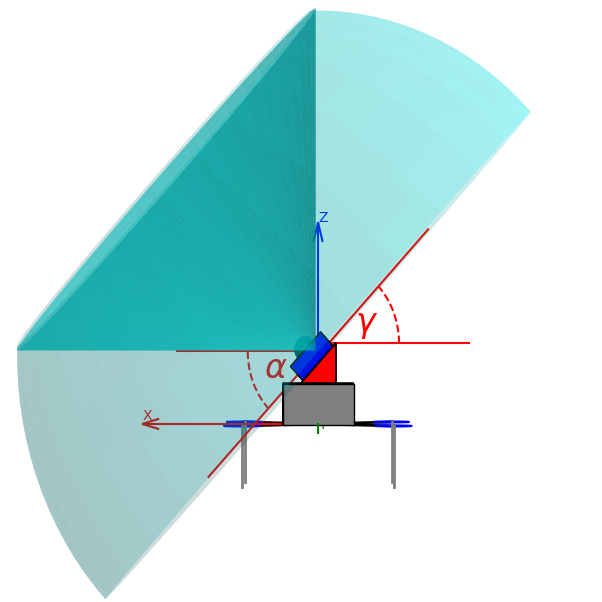
\includegraphics[width=0.48\textwidth]{./fig/photos/uav_side_view.png}
                \label{fig:model_uav}
                }
                \subfloat[UAV used in the experiment with mounted LiDAR] {
                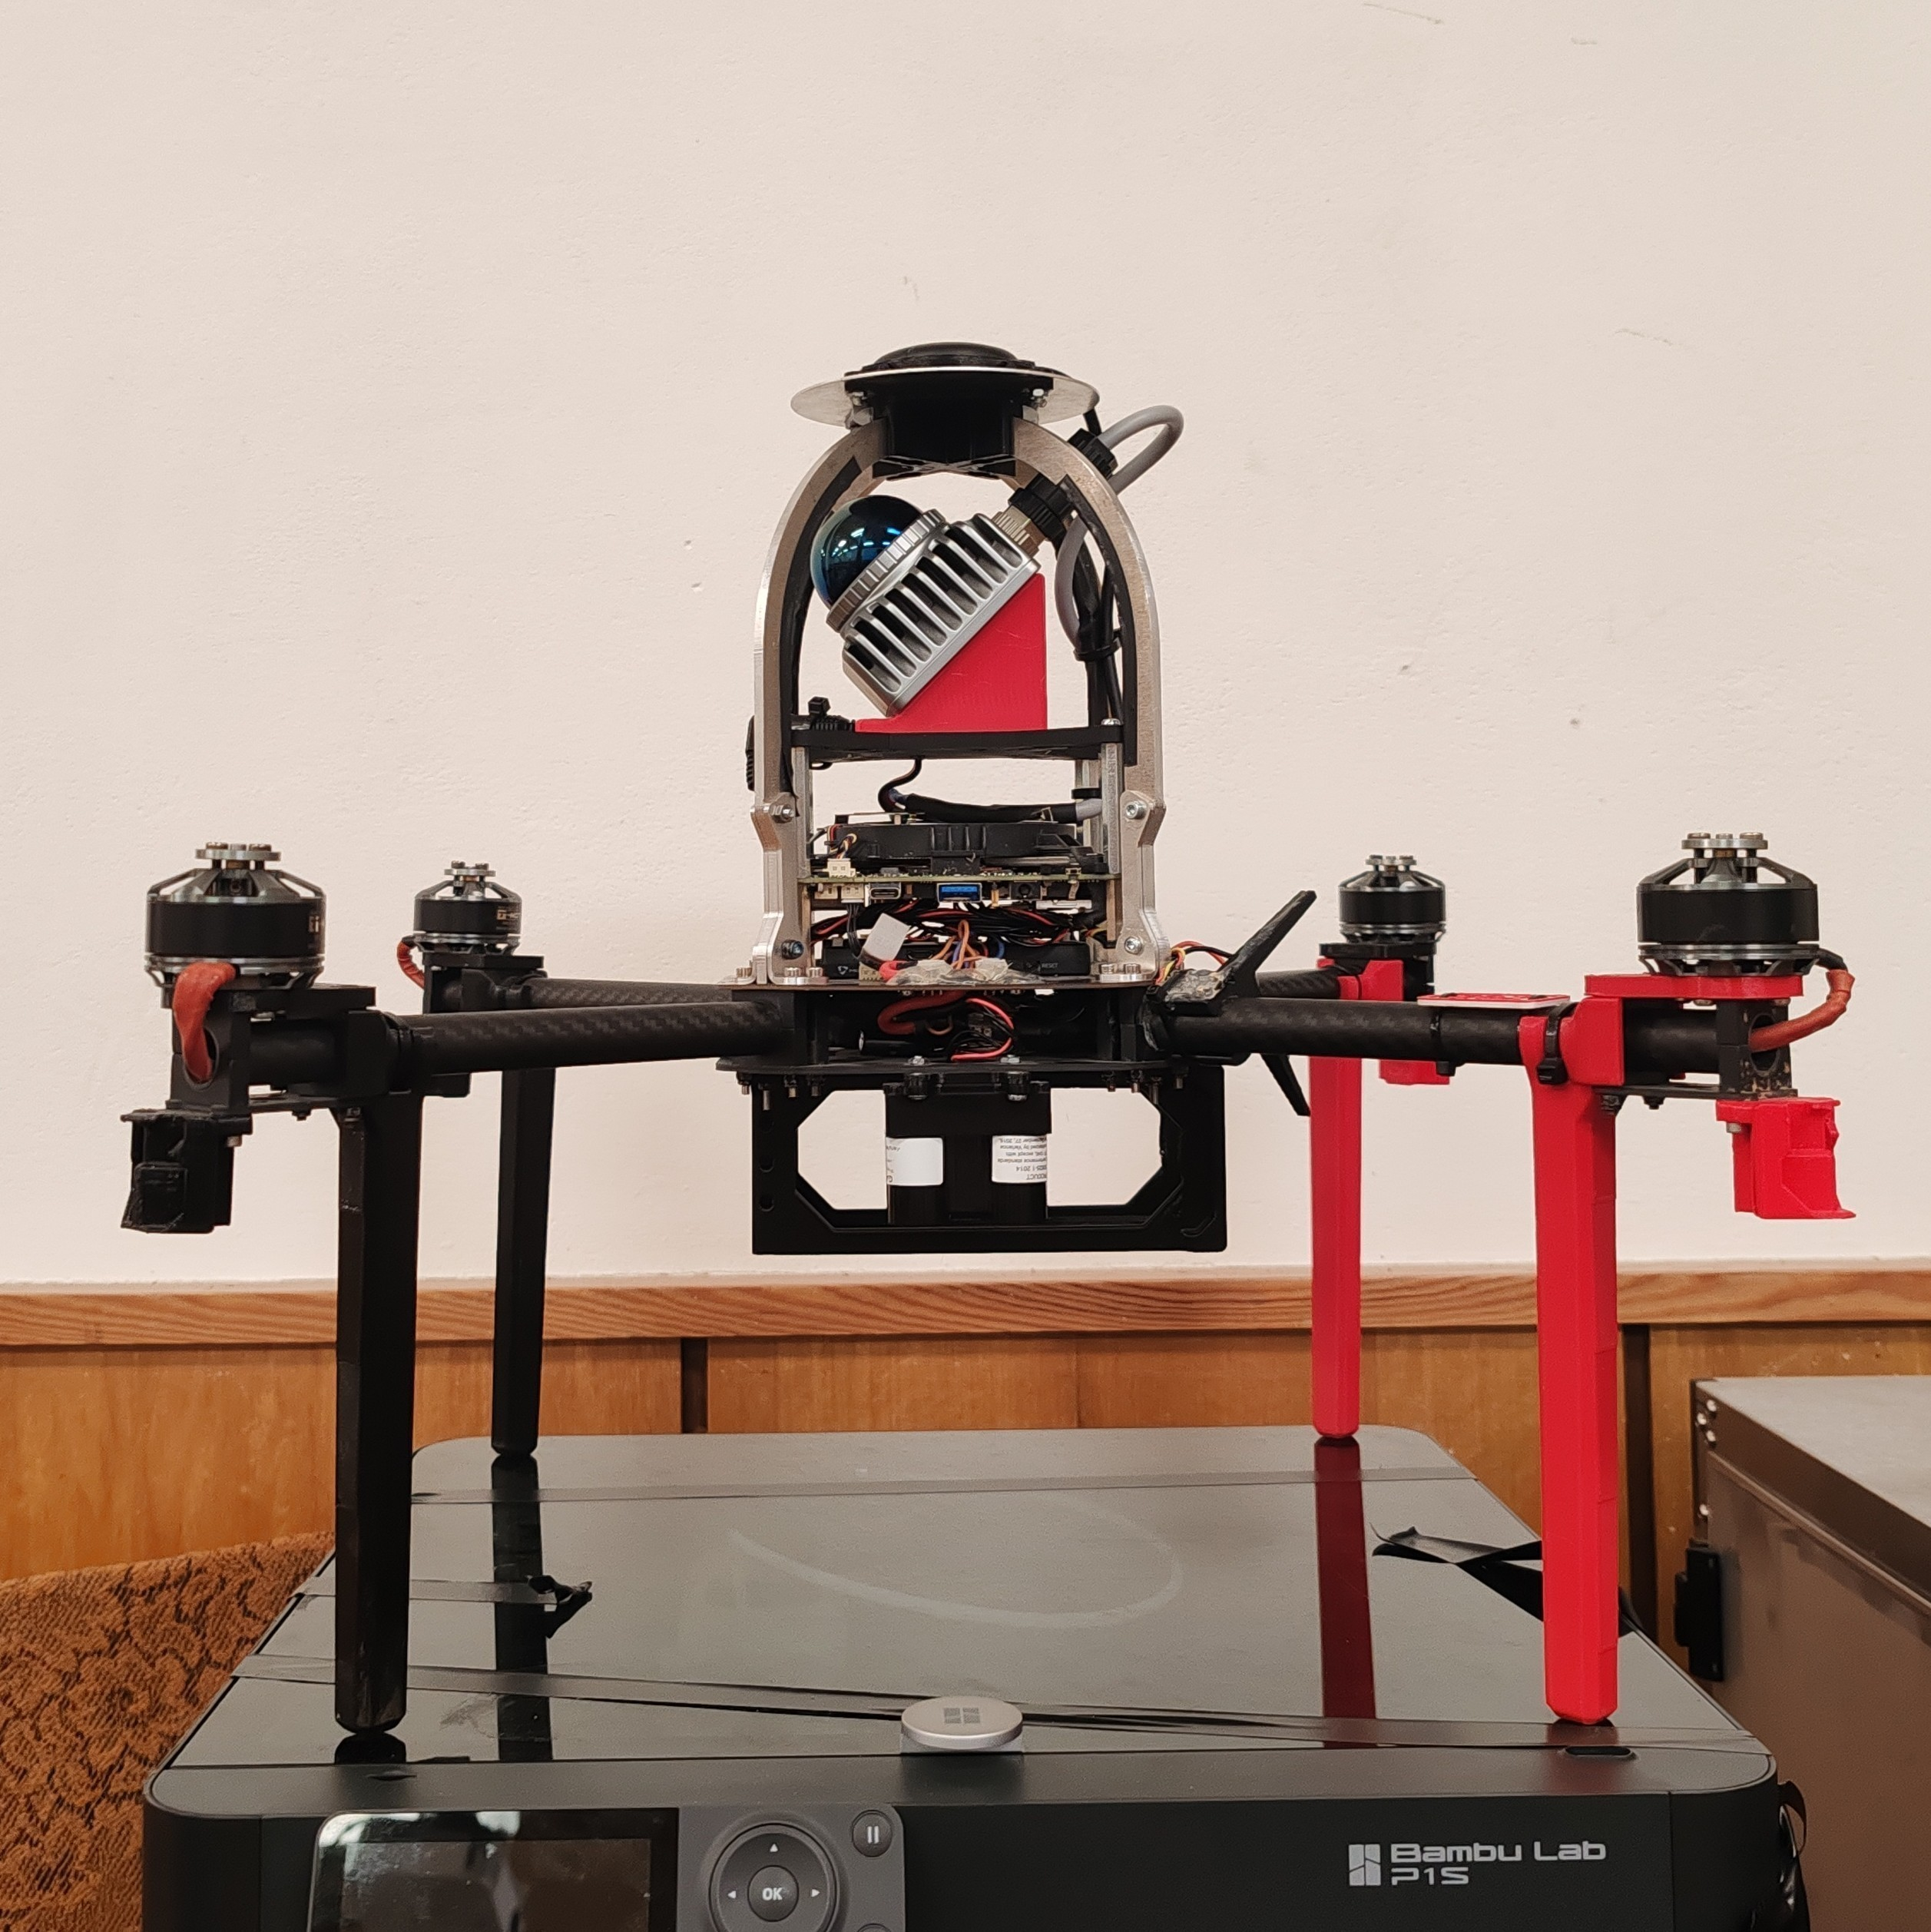
\includegraphics[width=0.48\textwidth]{./fig/photos/uav_photo.jpg}
                \label{fig:uav_1}
                }
                \caption{
                    UAV and LiDAR mounting scheme.
                    Subfigure (a) shows a modeled UAV with visualized LiDAR mounting parameters, including the LiDAR elevation field of view $\alpha$ and tilt angle $\gamma$. 
                    Subfigure (b) displays the real UAV used in the experiment with the LiDAR mounted according to the same configuration.                                                
                }
                \label{fig:uavs}
            \end{figure}

            For modification of cell A 2 planes are defined using real knowledge of how LiDAR is mounted on the uav and livox vertical fov
            Let $\mathbf{e}_z = \begin{bmatrix} 0 \\ 0 \\ 1 \end{bmatrix}$ be the unit vector along the z-axis,  
            $R_{\text{off}} \in SO(3)$ the offset rotation, and  
            $R_{\text{rpy}} \in SO(3)$ the roll-pitch-yaw rotation. 
            $\alpha_1$, $\alpha_2$, $\alpha_3$

            Then the resulting vector is given by:  
            \[
            \mathbf{n} = R_{\text{rpy}} \cdot R_{\text{off}} \cdot \mathbf{e}_z
            \]

            Modified cell S:
            \begin{equation}
                \mathcal{S}_i = {} 
            \end{equation}
            livox - 360 * 60 deg - account for centroid calculation
        \subsection{Software and Hardware setup}
            LiDAR sensor config, uav platform specifications
    
    \section{Simulation and Experimental Results}
        TODO
        \subsection{Simulation Setup}
            virtual environment modeling, tools used
        \subsection{Performance in Simulated Environments}
            Success rates, obstacle avoidance, efficiency metrics - same as in the rbl
        \subsection{Real-World Experiments in a Forest Environment}
        \subsection{Comparative Analysis}
            Simulation vs. real-world performance
    
    \section{Conclusion}
        TODO
        Summary of contributions and some directions for future research
    






















REDO after this

\section{Introduction}

Motivation for using 3d lidar and challenges

\section{3D LiDAR Sensor Model and Simulation Setup}

Overview of LiDAR used. Simulation configuration

\section{Object Detection and Approximation}

Methods for extracting objects from LiDAR point clouds. Approximating detected objects with simple shapes. Handling noisy or incomplete data

% \href{https://people.cs.umass.edu/~smaji/papers/pcagan.pdf}{Shape Generation using Spatially Partitioned Point Clouds by Gadelha et al.}

\href{https://groups.inf.ed.ac.uk/advr/papers/3D_Surface_Approximation_from_Point_Clouds.pdf}{3D Surface Approximation from Point Clouds} $\leftarrow$ This one seems promising. I would like to try this.

% \href{https://par.nsf.gov/servlets/purl/10347732}{Label-Efficient Learning on Point Clouds using Approximate Convex Decompositions by Gadelha et al.}

\href{https://en.wikipedia.org/wiki/Alpha_shape}{Alpha Shape: A Generalization of the Convex Hull}



\section{Integration with RBL Algorithm}

Modifications to ensure safe navigation and how approximated objects influence Voronoi cells

\section{Simulation Results}

Example scenarios - in rviz with drone and also in real life - me holding a branch with leafs or something like that

\section{Discussion}

Limitations and possible improvements

\section{Summary}